%%%%%%%%%%%%%
\chapter{Ergebnisdiskussion}
\label{ch:Results}
%%%%%%%%%%%%%
Zur Bewertung der Konzepte werden die in Kapitel \ref{ch:evaluation} beschriebenen Daten zunächst interpretiert. Die Ergebnisse der Interpretation werden anschließend kritisch betrachtet und, basierend auf der Ergebnisinterpretation, ein Ausblick der nächsten Schritte, für die Umsetzung des \emph{TMA} beschrieben. 


\section{Ergebnisinterpretation}
Die Ergebnisinterpretation erfolgt auf den, in Kapitel \ref{ch:evaluation}, aufgestellten Hypothesen. Ziel der Ergebnisinterpretation ist darzulegen, dass ein Modellierungsansatz nach dem Konfigurationsprinzip für den späteren Anwender verständlicher ist. Als Baseline dient hierfür das \emph{movisensXS}-System, welches ein Konstruktionsprinzip verfolgt. Dieser Ansatz bietet im Vergleich sehr viel Flexibilität in der Gestaltung einer Therapie. Die Ergebnisse werden kategorisiert betrachtet. Gegenübergestellt werden jeweils, wie bisher, das Konstruktionsprinzip und Konfigurationsprinzip, sowie der Einsatz von Sprüngen und die Verwendung von Sichtbarkeitsregeln. Die Betrachtung der Ergebnisse wird gemäß der zuvor verwendeten Reihenfolge erfolgen. Abschließend werden die Ergebnisse zusammengefasst dargestellt.


\subsection{Konfigurationsprinzip und Konstruktionsprinzip}
Eine erste Betrachtung der Ergebnisse, deutet darauf hin, dass die Nutzer die Umsetzung und Verwendung des Konfigurationsprinzips besser bewerteten als das Konstruktionsprinzip. Wie in Abbildung \ref{antwortendurchsch11} und Abbildung \ref{antwortendurchsch22} zu sehen ist, haben die Probanden den \emph{TherapyBuilder}-Prototyp im Schnitt besser bewertet als das angepasste \emph{movisensXS}-System. Diese Ergebnisse wurden den Zwischenfragebögen entnommen und zeigen eine erste Tendenz auf. 

Auch die Ergebnisse der Abschlussfragerunde geben einen ersten Hinweis auf die Bewertung der Verständlichkeit und Übersicht beider Prinzipien. Insgesamt konnten die Probanden in der Abschlussfragerunde achtundzwanzig Punkte nennen (vgl. Abbildung \ref{konstrabsch} und \ref{konfigabsch}), die ihnen am Konstruktionsprinzip gut gefallen haben und die sie besonders hilfreich empfanden. Zum Konfigurationsprinzip äußerten sie hierzu hingegen neununddreißig Punkte. Die Probanden konnten somit bezüglich des Konfigurationsprinzips insgesamt mehr Punkte äußern, die ihnen an dieser Umsetzung gut gefallen haben und besonders hilfreich empfunden wurden. Betrachtet man diese jedoch im Einzelnen, wurden Konstruktionsprinzip mehr Punkte dahingehend geäußert, was den Probanden gut gefallen hat. Hinsichtlich der Nachfrage, was den Probanden an der jeweiligen Umsetzung nicht gefallen hat und was sie vermisst haben, schnitt auch hier das Konfigurationsprinzip besser ab. Im Vergleich zum Konstruktionsprinzip fielen den Probanden neunzehn Punkte ein. Das sind dreizehn Punkte weniger als die Probanden zum Konstruktionsprinzip äußerten. Zwar gibt es insgesamt mehr positive Anmerkungen bezüglich des Konfigurationsprinzip, allerdings wurden gegenüber dem Konstruktionsansatz mehr Punkte genannt, die den Probanden an diesem Ansatz besonders gut gefallen haben. Welche Punkte das sind und wie sich diese mit den Ergebnissen und aufgestellten Hypothesen verbinden lassen, wird im Verlauf dieses Kapitels betrachtet.


\begin{figure}
   \begin{minipage}[b]{.49\linewidth} % [b] => Ausrichtung an \caption
      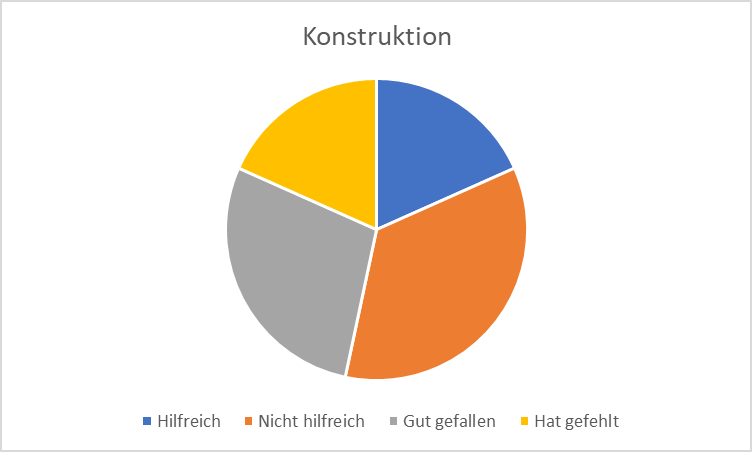
\includegraphics[width=\linewidth]{pictures/diagramme/aussagenkonstr}
      \caption{Zu sehen ist die Anzahl der genannten Punkte der Abschlussfragerunde. Die Probanden nannten achtundzwanzig Punkte auf die Frage was ihnen am Konstruktionsprinzip gut gefällt und sie als hilfreich empfinden}
      \label{konstrabsch}
   \end{minipage}
   \hspace{.01\linewidth}% Abstand zwischen Bilder
   \begin{minipage}[b]{.49\linewidth} % [b] => Ausrichtung an \caption
      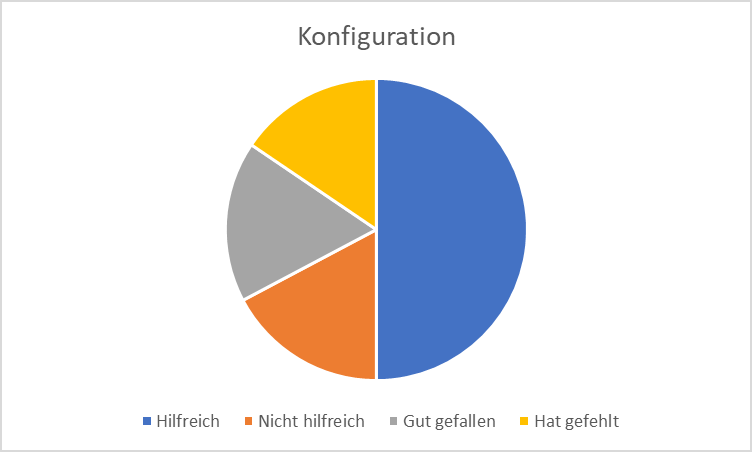
\includegraphics[width=\linewidth]{pictures/diagramme/aussagenkonfig}
      \caption{Im Vergleich äußerten die Probanden deutlich mehr Punkte, die sie am umgesetzten Konfigurationsprinzip als hilfreich empfinden. Allerdings konnten sie auch weniger Aussagen darüber treffen, was ihnen besonders gut gefallen hat}
      \label{konfigabsch}
   \end{minipage}
\end{figure}



\paragraph{Verständlichkeit der Triggereinstellungen}
Die Ergebnisse der Zwischenfragebögen zeigen eine Tendenz, dass im Vergleich das Kontruktionsprinzip für Anwender verständlicher ist. Die Freitexte der Zwischenfragebögen und Abschlussfragerunde deuten hingegen darauf hin, dass zwar viele Einstellungsmöglichkeiten geboten werden ohne mit diesen zu erschlagen und gefühlt weniger Einstellungsschritte und notwendig sind. Der Fluss vom Klicken wirkt klarer und konsistenter. Allerdings äußerten mehrere Probanden, dass die Einstellungen der Trigger zunächst irritierten. Betrachtet man die Ergebnisse der Abschlussfragerunde bestätigt sich letztere Aussage. Die Hälfte der Probanden wünschen sich eine Anleitung oder Tooltips zum besseren Verständnis der Triggereinstellungen.

Zwar wurde das \emph{movisensXS}-System im Zwischenfragebogen hinsichtlich der Triggereinstellungen schlechter bewertet. Dennoch kann das verwendete Konstruktionsprinzip mit seiner flexiblen Gestaltungsmöglichkeit aufwarten. Die Einstellungen der Trigger werden bei wachsender Komplexität unübersichtlicher. Aber insbesondere die vielen Einstellungsmöglichkeiten via Drag and Drop durch das Baukastenprinzip, und die Flexibilität in der Anordnung und Gestaltung, sind generell besser nachvollziehbar. Nicht nur das Baukastenprinzip und die einhergehende Drag and Drop Funktion tragen dazu bei, sondernm auch die Trennung verschiedener Elemente anhand ihrer Funktion. 

Insgesamt ist zwar eine Tendenz gegeben, dass das Konstruktionsprinzip leichter verständlich ist, allerdings benötigt dieses zusätzlich Anleitungen und Tooltips um diese zu verbessern. Auch wenn das Konstruktionsprinzip tendenziell schlechter abschneidet, so ist gerade das zusammenbauen der Triggereinstellungen für die Nutzer interessant und das Prinzip an sich leicht nachvollziehbar. Allerdings kann hier auch die flexible Anordnung zu einer geringeren Übersicht beitragen. Hier könnte eine automatische Anordnungsfunktion, oder Anordnungshilfe zur besseren Übersicht beitragen.


\paragraph{Verständlichkeit der Triggerdarstellung}
Auch hier lässt sich in Abbildung \ref{antwortendurchsch1} eine leichte Tendenz erkennen, dass die Triggerdarstellung im Konfigurationsprinzip verständlicher ist. Der Unterschied zwischen dem Konstruktionsprinzip und Konfigurationsprinzip ist hier allerdings relativ gering. Insbesondere die zeitliche Übersicht und das Zusammenbringen der Einstellungen und dem Ablauf empfanden die Probanden als positiv. Allerdings kristallisiert sich heraus, dass die Farben zwar zur Übersicht beitragen. Nur eine Erklärung dessen fehlt zum besseren Verständnis. Generell wurde die Darstellung zwar als übersichtlich beschrieben, aber die Verständlichkeit leidet unter den fehlenden Erläuterungen zu den angebotenen Farben, Symbolen und anderen Darstellungsformen. 

Das Konstruktionsprinzip hingegen wird zwar in der Darstellung schnell unübersichtlich, aber besonders die Farben der einzelnen Bausteine helfen beim Orientieren. Außerdem beinhaltet die Darstellung mehr Informationen auf einem Blick. Besonders die farbliche Kodierung der Blöcke wird von den Probanden positiv hervorgehoben. 

Zwar schneidet das Konfigurationsprinzip besser ab, allerdings nur geringfügig. das Konstruktionsprinzip hebt sich besonders durch die farbliche Kodierung hervor. Diese Eigenschaft kann sich das Konfigurationsprinzip zu eigen machen. Eine durchdachte farbliche Kodierung der Trigger in Kombination mit entsprechenden Symbolen und einer ausführlichen Legende mit Erklärungen, können erheblich zu einer verständlicheren Darstellung der Trigger beitragen. Auch das hinterlegen von Informationen über die Triggereinstellungen, in Form von Tooltips an den zeitlich dargestellten Elementen, können sich positiv auf das Konfigurationsprinzip auswirken. Auch hier kann das Konstruktionsprinzip von einer strikteren Anordnungsvorgabe profitieren. 

\paragraph{Übersichtlichkeit der Konversationen}
Betrachtet man die erhobenen Daten hinsichtlich der Übersichtlichkeit innerhalb der verschiedenen Konzepte, so lässt sich auch hier eine Tendenz erkennen. Wie in Abbildung \ref{antwortendurchsch22} zu sehen, schneidet das Konfigurationsprinzip des \emph{TherapyBuilders} besser in der Fragebogenauswertung ab als das Konstruktiosnprinzip. Die Tendenz zeigt, dass die Listendarstellung aller Konversationen innerhalb der Darstellung des Konfigurationsprinzip, übersichtlicher gestaltet ist, als die freie Anordnung innerhalb des Konstruktionsprinzips des \emph{movisensXS}. Die Ergebnisse der Abschlussfragerunde bekräftigen die Ergebnisse des Fragebogens. Besonders die Listendarstellung und die hierfür angebotene Suchmöglichkeit nach einzelnen Konversationen werden als positive Punkte angebracht. Diese wird im Konstruktionsprinzip hingegen vermisst. Will der Nutzer eine Konversation und dessen Triggereinstellungen betrachten, muss diese erst im Baum gesucht werden. 

Triggereinstellungen einer Konversation einzusehen, gestaltet sich im Konfigurationsprinzip tendenziell leichter. Eine Suchfunktion könnte das Konstruktionsprinzip in diesem Punkt verbessern.


\paragraph{Übersichtlichkeit der zeitlichen Darstellung der Konversationen}
Abbildung \ref{antwortendurchsch22} verdeutlicht die unterschiedliche Bewertung beider Systeme hinsichtlich ihrer zeitlichen Darstellung der Konversationen. Es zeichnet sich eine deutliche Tendenz ab, dass diese innerhalb des Konfigurationsprinzips eine bessere Übersicht über die zeitliche Steuerung der Konversationen besteht. Die Ergebnisse der Freitexte, sowie der Abschlussfragerunde, untermauern das Ergebnis. So ist der zeitliche Ablauf und die Darstellung im Zeitstrahl übersichtlich, leicht nachvollziehbar. Außerdem lässt sich die spätere Belastung des Patienten einsehen. Alle Probanden äußerten sich positiv über diese Art der Darstellung. Ein Proband vermisst allerdings Funktionen bei dieser Darstellung. So wünscht sich dieser eine Möglichkeit auf einzelne Elemente zu klicken und eine Funktion damit auszulösen. Hingegen wurde das Konstruktionsprinzip in diesem Punkt ausschließlich kritisiert. Der zeitliche Ablauf der Konversationen ist schwer zu überblicken. 

Das Konfigurationsprinzip kann leicht um den Punkt der klickbaren Elemente und einer dahinter versteckten Funktion, wie beispielsweise das Aufrufen der Trigger-Einstellungen, erweitert werden. Um das Konstruktionsprinzip in diesem Punkt zu verbessern, könnte eine stärkere Vorgabe für die Strukturierung und Anordnung der Elemente auf dem entsprechenden Arbeitsblatt hilfreich sein. So könnte auch eine zeitliche Abfolge der Konversationen dargestellt werden.


\paragraph{Verständlichkeit der Triggerkonfiguration}
Hinsichtlich der Konfigurierung der Trigger wurde der \emph{TherapyBuilder}-Prototyp schlechter bewertet als der \emph{movisensXS}-Prototyp. Es ist eine Tendenz erkennbar, die aufzeigt, dass das Konstruktionsprinzip hinsichtlich der Triggerkonfiguration verständlicher ist. Die Betrachtung der Freitext-Aussagen sowie der Abschlussfragerunde geben Hinweise, in welchen Punkten sich das Konstruktionsprinzip hervorhebt. So ist insbesondere die Anordnung der Bausteine leicht verständlich. Die Drag and Drop Funktion erleichtert diese außerdem. Die einhergehende Flexibilität der Anordnung, sowie die farbliche Kodierung der Bausteine fallen positiv auf und tragen der Verständlichkeit bei. Diese wird beim Konfigurationsprinzip vermisst. So sind die Einstellungen der Konditionen nicht ganz klar. Außerdem lässt sich die Bearbeitungsfunktion der Trigger schwer finden. 

Um die Konfiguration der Trigger des Konfigurationsprinzip verständlicher zu gestalten, benötigt es zunächst einen besseren Zugang zu den Einstellungen. Außerdem sollten die Funktionen und Einstellungen erneut überarbeitet werden. Hier könnte eine strengere Form des Konstruktionsprinzips verwendet werden um die Einstellungsmöglichkeiten flexibel und verständlich zu gestalten. Möglich wäre eine Vorgabe von kleinen Bausteinen, die beliebig angeordnet, farblich kodiert und eingestellt werden können, sich allerdings nur auf eine Konversation bezieht, statt, wie im Konstruktionsprinzip, auf beliebig viele. Diese Form könnte die Übersichtlichkeit des Konfigurationsprinzip beibehalten.


\paragraph{Verständlichkeit von Abhängigkeiten zwischen Konversationen und Konversationsverzweigungen}
Die Abhängigkeiten zwischen Konversationen ist im Vergleich zum 
Die Grafiken \ref{antwortendurchsch11} und \ref{antwortendurchsch22} verdeutlichen eine positive Tendenz hinsichtlich der Verständlichkeit von Konversationsverzweigungen und Abhängigkeiten zwischen Konversationen im \emph{TherapyBuilder}. Das dort eingesetzte Konfigurationsprinzip wird in diesem Punkt allerdings kaum in den Freitext-Aussagen sowie der Abschlussfragerunde erwähnt. Nur zwei Probanden äußern, dass die Darstellung der Abhängigkeiten gut einsehbar sind. Der \emph{movisensXS}-Prototyp wird generell als weniger übersichtlich und verständlich bezüglich des zeitlichen Verlaufs beschrieben. Allerdings geht auch hier kein Proband genauer auf die Abhängigkeiten zwischen Konversationen ein. 

Generell könnte das Konstruktionsprinzip des \emph{TherapyBuilder} auch in diesem Punkt durch eine verständliche und ausführliche Legende, sowie Tooltips mit entsprechenden Informationen, die Verständlichkeit der Abhängigkeiten verbessern. Das Konstruktionsprinzip könnte auch hier von einer strikteren Anordnungsvorgabe profitieren. 

\paragraph{Übersichtlichkeit der Therapie}

%Insgesamt empfanden die Probanden die Übersichtlichkeit der Therapie und deren Verlauf als eher mäßig. Ein Proband gab an, dass die Therapie für ihn schlecht zu überschauen ist. Die restlichen Probanden hingegen bewerteten diese zwischen sehr gut bis eher gut. Dies spiegelt sich wiederum in der Aussage über die fehlende Übersichtlichkeit innerhalb der Baum-Darstellung wieder. Dies wurde - wie bereits erwähnt - von der Hälfte der Probanden angemerkt. 

%Im Gesamten wurde die Übersichtlichkeit der Therapie innerhalb des Konfigurationsprinzips als gut bewertet. Wobei sich hier eine leichte Tendenz zu sehr gut andeutet. Dies lässt sich auch aus den Freitext-Aussagen der Probanden ableiten. Hundert Prozent der Probanden gaben an, dass die Darstellung der Therapie in Form einer Timeline übersichtlich ist und ihnen gut gefallen hat. Außerdem lässt sich der gesamte Therapieverlauf gut ableiten.





\subsection{Sprünge und Sichtbarkeitsregeln}

\begin{figure}
   \begin{minipage}[b]{.49\linewidth} % [b] => Ausrichtung an \caption
      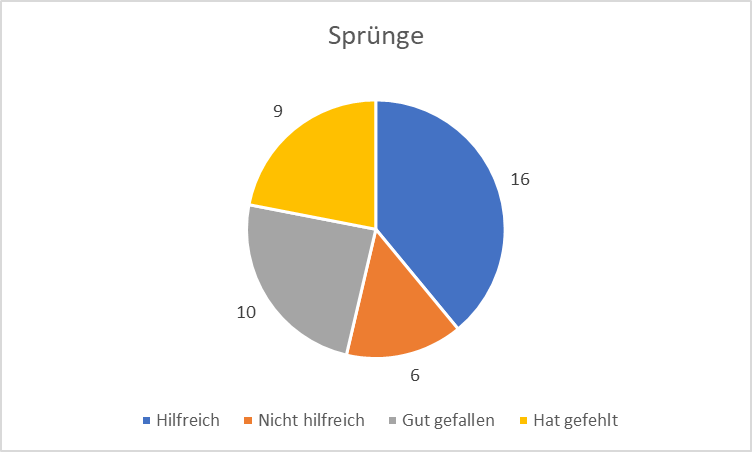
\includegraphics[width=\linewidth]{pictures/diagramme/aussagenspr}
      \caption{Wasser}
   \end{minipage}
   \hspace{.01\linewidth}% Abstand zwischen Bilder
   \begin{minipage}[b]{.49\linewidth} % [b] => Ausrichtung an \caption
      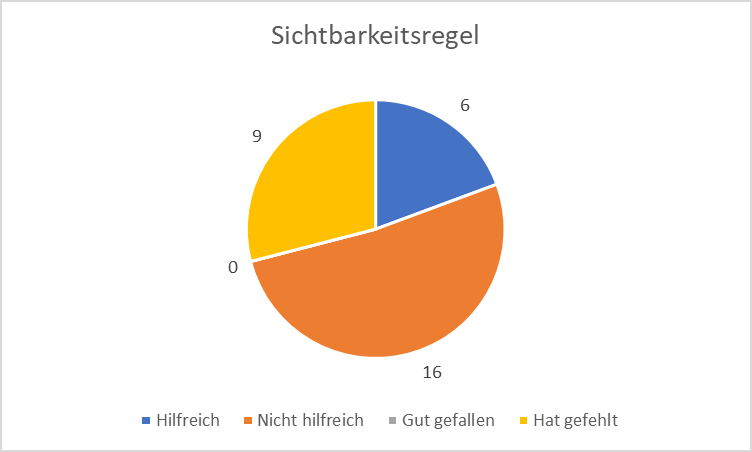
\includegraphics[width=\linewidth]{pictures/diagramme/aussagensichtb}
      \caption{Land}
   \end{minipage}
\end{figure}

\paragraph{Verständlichkeit der Konversationsdarstellung}

\paragraph{Verständlichkeit der Konversationseinstellungen}

\paragraph{Übersichtlichkeit des Konversationsverlaufs}

\paragraph{Übersichtlichkeit der Antwortoptionen innerhalb des Konversationsverlaufs}

\paragraph{Verständlichkeit der Verzweigungen innerhalb des Konversationsverlaufs}

\paragraph{Übersichtlichkeit der Werkzeugpalette zur Konversationserstellung}




\subsection{Zusammenfassung}

\section{Kritische Reflexion}

\begin{figure}[h]
\centering
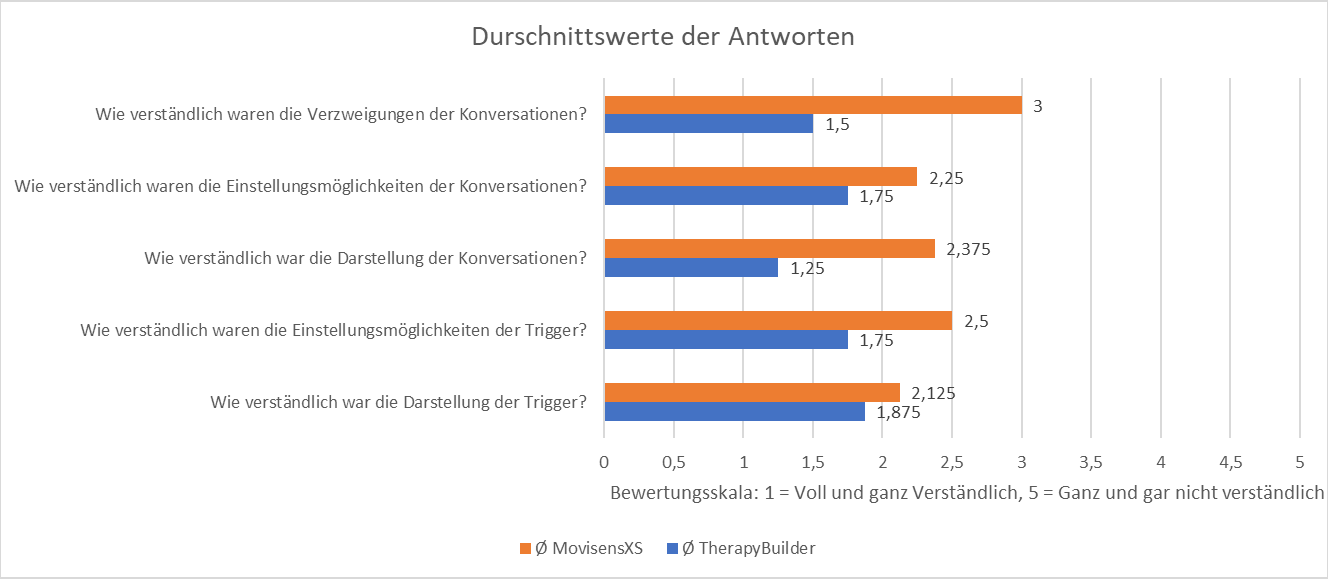
\includegraphics[width=1\textwidth]{pictures/diagramme/antwortendurchsch1}
\caption{Architektur des \emph{konfiguration}}
\label{antwortendurchsch11}
\end{figure}

\begin{figure}[h]
\centering
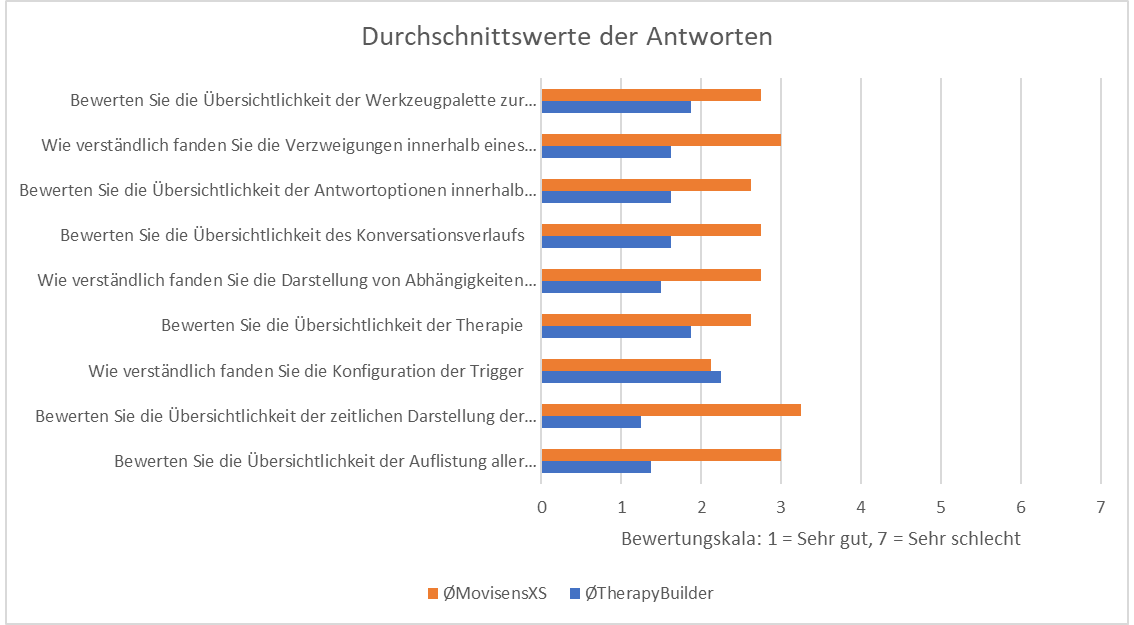
\includegraphics[width=1\textwidth]{pictures/diagramme/antwortendurchsch2}
\caption{Architektur des \emph{konfiguration}}
\label{antwortendurchsch22}
\end{figure}


%Ziel der Arbeit ist die Konzeption eines Therapiemodellierungsansatz (\emph{TMA}). Dieser soll es erlauben, auch technisch wenig versierten Psychologen ihre Therapieideen in einer Art und Weise zu formulieren, die von einer Maschine verarbeitet und ausgeführt werden kann. Dadurch entfällt der hohe und fehleranfällige Abstimmungsaufwand zwischen Forschern und Entwicklern. 


%%%%%%%%%%%%%%%%%%%%%%%%%%%%%%%%%%%%%%%%%%%%%%%%%%%%%%%%%%%%%%%%%%%%%
%%%%%%%%%%%%%%%%%%%%%%%%%%%%%%%%%%%%%%%%%%%%%%%%%%%%%%%%%%%%%%%%%%%%%

%\paragraph{Verständlichkeit der Triggerdarstellung}
%Die im Konfigurationsprinzip verwendete grafische Abbildung der zeitlichen Abläufe, durch Zeitstrahl, farbliche Kodierung, Symbole und Anordnung der Konversationen als Liste verdeutlicht, wirken sich positiv auf die Verständlichkeit der Triggerdarstellung aus. 
%
%Im Vergleich steht das Konstruktionsprinzip, welches die Triggerdarstellung als zeitliche Abläufe grafisch, als Baum und durch die Anordnung von Blöcken, wie Konversationen (Conversations), Auslösern (Triggern) und Bedingungen (Conditions) sowie einer farblicher Kodierung, nach dem Ampelprinzip, und Formen umsetzt.
%
%
%\paragraph{Verständlichkeit der Triggereinstellungen}
%Die direkte Bindung von Bedingungen (Conditions) und Auslösern (Triggern) sowie deren Einstellungen an eine Konversation wirkt sich positiv auf die Verständlichkeit der Triggereinstellungen aus. 
%
%Dem entgegen steht die Anordnung von Auslösern (Triggern) und Bedingungen (Conditions) in Verschachtelungen, mit beliebig vielen Bezügen zu Konversationen.
%
%\paragraph{Übersichtlichkeit der Konversationen}
%Die Darstellung aller vorhandenen Konversationen in Form einer Liste, innerhalb der zeitlichen Darstellung, trägt zur Verbesserung der Übersichtlichkeit der Verwendeten Konversationen bei.
%
%Innerhalb des Konstruktionsprinzips wird die Darstellung aller verwendeten Konversationen, im Samplingbaum in Form von \emph{Conversation}-Blöcke umgesetzt. Diese können beliebig im Baum platziert und angeordnet werden.
%
%\paragraph{Übersichtlichkeit der zeitlichen Darstellung der Konversationen}
%Die im Konfigurationsprinzip verwendete grafische Abbildung der zeitlichen Abläufe, in Form eines Zeitstrahls und durch Anordnung der Konversationen als Liste, trägt zu einer besseren Übersicht der zeitlichen Abfolge von Konversationen bei. 
%
%Im Vergleich steht das Konstruktionsprinzip, welches die zeitliche Abläufe grafisch, als Baum und durch die Anordnung von Blöcken, wie Konversationen (Conversations) und Auslösern (Triggern), umsetzt.
%
%\paragraph{Verständlichkeit der Triggerkonfiguration}
%Die Art der Unterscheidung zwischen Trigger und Condition tragen zur Verständlichkeit der Konfiguration der Triggereinstellungen einer Konversation bei. Hierbei gibt es zwischen Trigger und Condition keine Abhängigkeit. 
%
%Im Gegensatz zum Konfigurationsprinzip setzt das Konstruktionsprinzop eine Unterscheidung zwischen Trigger und Condition innerhalb des Samplingbaums ein. Diese werden durch Blöcke dargestellt, die sich in Farbe, Form und Anordnungsmöglichkeit unterscheiden. Trigger und Conditions sind außerdem voneinander abhängig.
%
%\paragraph{Übersichtlichkeit der Therapie}
%Insgesamt tragen die Verwendeten Stilmittel des Konfigurationsprinzip, zur Übersichtlichkeit einer Therapie, bei. Die Verwendeten Stilmittel sind hierbei die Auflistung der Verwendeten Konversationen, die zeitliche Darstellung dieser in einem Zeitstrahl, Unterscheidung dieser anhand von Farben und Formen sowie Verdeutlichung von Abhängigkeiten zwischen Konversationen durch Linien. 
%
%Dieser Form der Übersicht steht die Darstellung der Therapie in Form eines Baums entgegen. Die Übersicht der Therapie wird hierbei durch Anordnung der Blöcke, deren Farben sowie Inhalte, Verbindungen und Anordnung gegeben. 
%
%
%\paragraph{Verständlichkeit von Abhängigkeiten zwischen Konversationen und Konversationsverzweigungen}
%Die Abbildung der Abhängigkeiten zu anderen Konversationen im Zeitstrahl und der Verzweigung von Konversationen, visualisiert durch Linien, wirkt sich positiv auf die Verständlichkeit von Verzweigungen von Konversationen und Abhängigkeiten zwischen Konversationen aus. 
%
%Diesem Designprinzip steht die Darstellung von  Abhängigkeiten zu anderen Konversationen durch Verzweigungen im Baum und \emph{Check Variable} Blöcke entgegen. 


%%%%%%%%%%%%%%%%%%%%%%%%%%%%%%%%%%%%%%%%%%%%%%%%%%%%%%%%%%%%%%%%%%%%%
%%%%%%%%%%%%%%%%%%%%%%%%%%%%%%%%%%%%%%%%%%%%%%%%%%%%%%%%%%%%%%%%%%%%%


%\subsubsection{Sprünge und Sichtbarkeitsregeln}
%Die verwendeten Sprünge und damit einhergehende Darstellung, wird hinsichtlich dessen Verständlichkeit und Übersichtlichkeit überprüft. Aufgestellt werden Hypothesen, die auf die Darstellung und Einstellung einer Konversation eingehen. Insgesamt werden zum Konzept der Sprünge und dessen Umsetzung sechs Hypothesen aufgestellt, die eine Verbesserung gegenüber der Verwendung von Sichtbarkeitsregeln und der zugehörigen Darstellung messen sollen.
%
%\paragraph{Verständlichkeit der Konversationsdarstellung}
%Die Darstellung einer Konversation, welche mit dem Einsatz von Sprüngen einhergeht, trägt zur besseren Verständlichkeit der Konversationsdarstellung bei. In der Umsetzung werden Chatverläufe in einer Weise dargestellt, die in bekannten Chat-Technologien zum Einsatz kommt. Dies beinhaltet räumliche wie farbliche Trennung der Chatbot-Ausgaben und Nutzer-Eingaben.
%
%Dieser Form der Umsetzung wird die Unterscheidung durch Icons und Textbeschreibung entgegen gestellt.
%
%
%\paragraph{Verständlichkeit der Konversationseinstellungen}
%Das Einbauen eines Elements, welches Variablen überprüft und sich auf mehrere Elemente auswirken kann, trägt zur besseren Verständlichkeit der Einstellung des Konversationsverlaufs bei.
%
%Das Konzept der \emph{Sichtbarkeitsregeln}, welches entgegen gestellt wird, nutzt die Metapher eines Auges. Dieses kann an einer Form aktiviert werden um eine Sichtbarkeitsregel zu hinterlegen. Die Sichtbarkeitsregel bezieht sich nur auf die entsprechende Form. 
%
%\paragraph{Übersichtlichkeit des Konversationsverlaufs}
%Die Verwendung von Spalten, sogenannten \emph{Lanes}, tragen zur Übersicht von Konversationsverzweigungen bei.
%
%
%\paragraph{Übersichtlichkeit der Antwortoptionen innerhalb des Konversationsverlaufs}
%Die Visualisierung von Nutzereingabe innerhalb der Dialogansicht durch den Einsatz der Button-Metapher trägt zur besseren Übersicht der Antwortmöglichkeiten des Nutzers bei.
%
%Diesem Konzept steht die Darstellung der Antwortmöglichkeiten nach öffnen der Einstellungen einer Form entgegen.
%
%
%\paragraph{Verständlichkeit der Verzweigungen innerhalb des Konversationsverlaufs}
%Die Visualisierung von Verzweigungen innerhalb eines Dialogverlaufs mittels Bedingungsblock und Verweis auf Lanes, tragen maßgeblich zur Verständlichkeit bei. Der Nutzer versteht, dass es sich um eine Verzweigung handelt und welche Auswirkungen diese hat. 
%
%Diesem Design steht die Visualisierung von Verzweigungen innerhalb eines Dialogverlaufs mit Sichtbarkeitsregeln entgegen.



%\paragraph{Übersichtlichkeit der Werkzeugpalette zur Konversationserstellung}
%Eine strikte Trennung von Chatbot-Ausgabe und Nutzereingabe trägt maßgeblich zur Übersichtlichkeit der Werkzeugpalette bei. 
%
%Dem steht die Trennung von Chatbot-Ausgabe ohne Erwartung eines Nutzerinputs und Chatbot-Ausgaben mit Erwartung eines Nutzerinputs entgegen, die im \emph{movisensXS}-Prototyp verwendet wird. 

%Dieses Konzept wurde ebenfalls von den Probanden bewertet. Aus der Bewertung lassen sich folgende Aussagen treffen. 

%Auf Basis der Sichtbarkeitsregel und dem Design des Konversationsverlaufs wurde die Darstellung der Konversationen generell als zumeist verständlich bewertet. Es lässt sich eine leichte Tendenz erkennen, die angibt, dass die Darstellung zum Teil verständlich ist. Die Probandenaussagen der Freitexte untermauern die Bewertung. Es wurden bezüglich der Darstellung keine Punkte genannt, die den Probanden besonders positiv hervorstach. Hingegen wurden mehrere Aussagen getroffen, welche die Darstellung der Konversationen bemängeln. Etwas mehr als sechzig Prozent der Nutzer haben sich diesbezüglich negativ geäußert.

%Die Einstellungmsöglichkeiten der Konversationen wurde von den Probanden ebenfalls als zumeist verständlich, mit leichter Tendenz zu zum Teil verständlich, wahrgenommen. Hier wurde in knapp achtunddreißig Prozent der Aussagen die Vielfalt der Einstellungsmöglichkeiten positiv hervorgehoben. Auch die Kategorisierung der Einstellungsmöglichkeiten wurde einmal positiv erwähnt. Hingegen wurde ebenfalls in achtunddreißig Prozent der Aussagen die Unterscheidbarkeit zwischen Chatbot-Output und Patient-Input Elementen, innerhalb des Werkzeugkastens, bemängelt. Diese unterscheiden sich kaum. 

%Als gut, mit starker Tendenz zu eher gut, wurde im Schnitt die Übersichtlichkeit des Konversationsverlaufs bewertet. Vier der Freitextaussagen bemängeln die Übersicht der Konversationen. Zum einen sei der zeitliche sowie der generelle Verlauf schwer nachvollziehbar.

%Die Übersichtlichkeit der Antwortoptionen innerhalb eines Konversationsverlauf wurden von den Probanden im Schnitt als gut empfunden. Die durchschnittliche Bewertung weist dabei eine starke Tendenz zu \emph{eher gut} auf. Dies lässt sich auch in den schriftlichen Aussagen der Probanden wiederfinden. Vier Aussagen äußern sich negativ zur Darstellung des Verlaufs. Keine Aussage geht speziell auf die Antwortoptionen ein. 

%Als eher gut bewerteten die Probanden im Schnitt die Verständlichkeit der Verzweigungen innerhalb einer Konversation. Hierzu passen die Freitext-Aussagen der Probanden, die angaben, dass die Übersicht des zeitlichen Verlaufs fehle und somit für diese Probanden eher schwer nachvollziehbar ist. Diese Aussage trafen fünfzig Prozent. Ein Proband wies außerdem darauf hin, dass ihm unklar ist, woher die Variable stammt, die für die Verzweigung überprüft wird. 

%Im Schnitt bewerteten die Probanden die Übersichtlichkeit der Werkzeugpalette zur Erstellung des Konversationsverlaufs als gut. Auch hier zeigte sich eine starke Tendenz zur schlechteren Bewertung. Hier merkte ein Probanden an, dass der Zustand der Werkzeugpalette beim Öffnen des Konversationsreiters, hinderlich ist. Die Einstellungsmöglichkeiten des Chatbot-Outputs sind durch diesen leicht zu übersehen. 